\section{Introducción}
\label{sec:aim}

\subsection{Contexto y justificación}
\label{subsec:context}

La virtualización no es nada nuevo. Tiene sus orígenes en la respuesta de IBM al pryecto MAC (originalmente \emph{Mathematics and Computation}, renombrado más tarde a \emph{Multiple Access Computer}), que pretendía soportar más de un usuario de forma simultánea. Aunque los sistemas de hoy en día soportan cargas de trabajo multiusuario sin ningún problema, en aquellos tiempos cada usuario realizaba su computación en lotes secuenciales.

Para hacer realidad ése proyecto, el MIT necesitaba un hardware más potente del cual disponían, y se acercó a diferentes fabricantes. El proceso culminó con la elección  de GE como proveedor, ya que IBM no veía futuro en \emph{mainframes} concurrentes. Ésta oportunidad perdida sirvió para que IBM reaccionara, que a raíz de ello inició a desarrollar el CP-40, que acabaría llevando al CP-67, el primer mainframe que soportaba virtualización.

De todas formas, la virtualización aplicada a servicio pasó a un segundo plano a causa de la evolución meteórica de la informática durante los años 80 y 90, aademás del relativo bajo precio de servidores basados en la arquitectura x86. Con el paso del tiempo, fueron surgiendo diferentes soluciones de virtualización de escritorio, pero el modelo de computación distribuida se estableció como el estándar de la industria.

Actualmente, los servidores de La Bastida están todos implementados en un único servidor físico. Aunque esto funciona bien, constituye un \emph{SPOF} que en caso de fallar, dejaría al centro sin servicio. Éste proyecto, entonces, tiene por objetivo explorar el uso de la virtualización para mantener a flote los servicios en caso de que el servidor que los provee falle.

\subsection{Objetivos}
\label{subsec:objectives}

Los objetivos principales del proyecto son:

\begin{itemize}
    \item Estudiar y conocer el Apache Cassandra.
      \begin{itemize}
      \item Identificar los usos ideales para Apache Cassandra.
      \end{itemize}
    \item Entender el modelo de datos y consultas de Apache Cassandra.
    \item Diseñar un sistema para almacenar estadísticas sobre el tráfico de red
      en Apache Cassandra.
    \item Entender y familiarizarse con el flujo de trabajo del \emph{data scientist}.
      \begin{itemize}
      \item Analizar mediante Python los datos obtenidos de Cassandra, y
        intentar predecir el tráfico de red en el futuro.
      \end{itemize}
\end{itemize}

\subsection{Metodología}
\label{subsec:metodologia}

El proyecto se dividirá en dos partes bien diferenciadas: la primera consistirá
de un estudio de las bases de datos NoSQL, en concreto Apache Cassandra, y una
comparativa en base al modelo relacional.

La segunda, consistirá en emplear lo aprendido en la primera parte para
implementar un sistema que aproveche las aptitudes de Cassandra para el
\emph{big data} y el análisis de datos. A éstos efectos, se utilizará Python y
un variado conjunto de librerías para explorar los datos recogidos,
visualizarlos, y intentar predecir el tráfico de red estimado en un punto
concreto del futuro.



\subsection{Planificación del proyecto}
\label{subsec:planificació}

% \subsubsection{Lista de tareas}
% \label{subsubsec:tasklist}

% \includegraphics[page=4,scale=0.75]{salida.pdf}
% 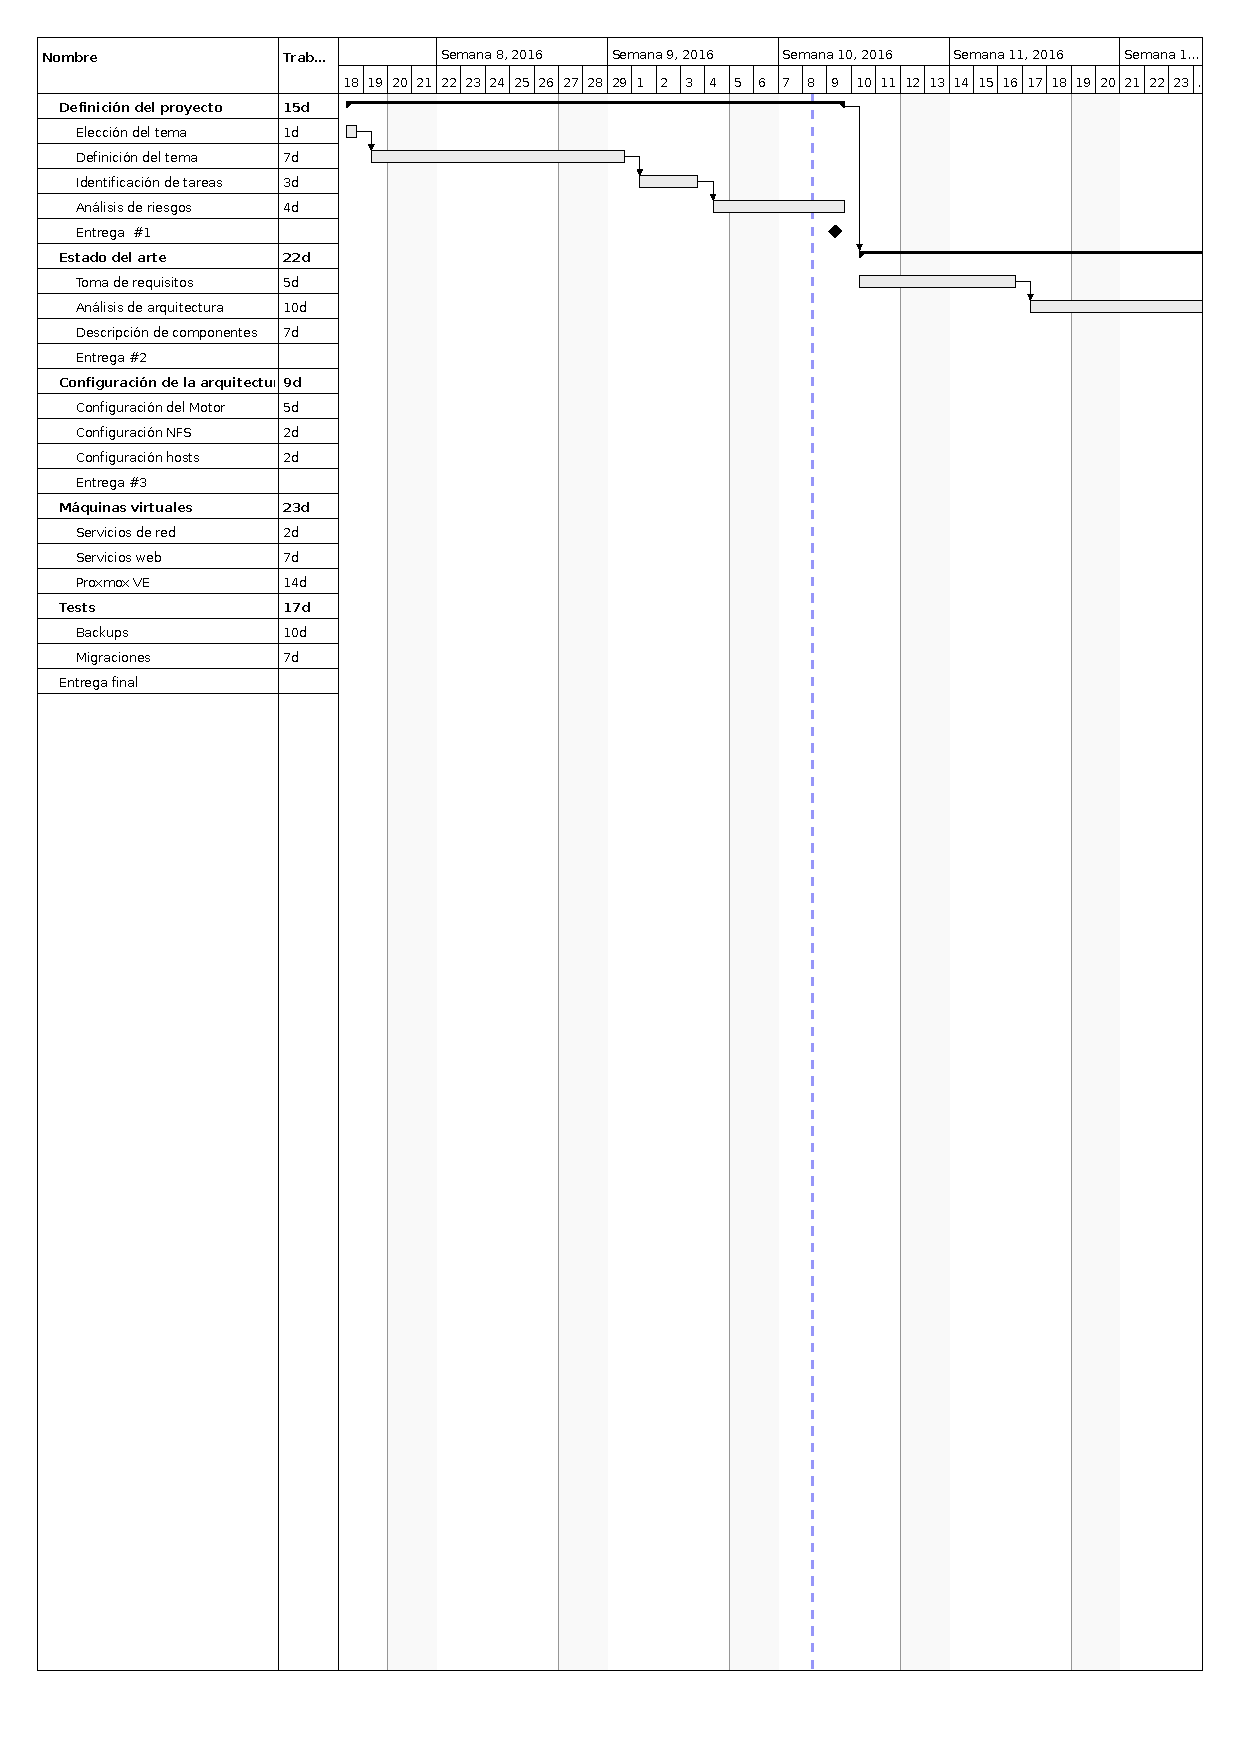
\includepdf[pages={1-3},scale=0.70]{salida.pdf}

\subsubsection{Planificación horaria}
\label{subsubsec:hores}

Debido a que el hardware necesario para la realización del proyecto se encuentra en el IES La Bastida (Nota: aunque en el anexo hay documentada una manera de acceder a la consola de administración a través de un proxy SOCKS, una retahíla de errores y descalabros a nivel físico han hecho muy difícil el trabajo de manera remota.) únicamente dispondré de tres horas durante los días lectivos para la realización del proyecto. El resto de horas del MP14 se dedicarán a investigar documentación, redactado de la memoria, y tareas relacionadas con la memoria y la presentación del proyecto.

A eso de Mayo de 2016, entré a trabajar para Coopux Systems, lo que me impide continuar cualquier tipo de trabajo en el proyecto. Por suerte, oVirt ya había sido probado y documentado, así que el impacto en el proyecto es relativamente pequeño, limitándose a la imposibilidad de documentar otras herramientas, y profundizar en la migración de máquinas virtuales.

\subsection{Descripción de los capítulos}
\label{subsec:chaps}

\begin{enumerate}
    \item \textbf{Estado del arte: } En éste capítulo se analizará la historia y el estado actual de la virtualización, se estudiará la arquitectura actual de La Bastida, y mi propuesta para el cambio.
    \item \textbf{Implementación de oVirt: } En éste capítulo, se documentará el proceso de instalación de oVirt.
    \item \textbf{Trabajando con VMs en oVirt: } En éste capítulo se documentará brevemente algunas de las tareas esenciales a la hora de trabajar con máquinas virtuales
    \item \textbf{Conclusiones: } En éste capítulo se resumirán mis conclusiones y opiniones personales acerca del proyecto.
\end{enumerate}
\clearpage
